
%% bare_jrnl.tex
%% V1.3
%% 2007/01/11
%% by Michael Shell
%% see http://www.michaelshell.org/
%% for current contact information.
%%
%% This is a skeleton file demonstrating the use of IEEEtran.cls
%% (requires IEEEtran.cls version 1.7 or later) with an IEEE journal paper.
%%
%% Support sites:
%% http://www.michaelshell.org/tex/ieeetran/
%% http://www.ctan.org/tex-archive/macros/latex/contrib/IEEEtran/
%% and
%% http://www.ieee.org/



% *** Authors should verify (and, if needed, correct) their LaTeX system  ***
% *** with the testflow diagnostic prior to trusting their LaTeX platform ***
% *** with production work. IEEE's font choices can trigger bugs that do  ***
% *** not appear when using other class files.                            ***
% The testflow support page is at:
% http://www.michaelshell.org/tex/testflow/


%%*************************************************************************
%% Legal Notice:
%% This code is offered as-is without any warranty either expressed or
%% implied; without even the implied warranty of MERCHANTABILITY or
%% FITNESS FOR A PARTICULAR PURPOSE! 
%% User assumes all risk.
%% In no event shall IEEE or any contributor to this code be liable for
%% any damages or losses, including, but not limited to, incidental,
%% consequential, or any other damages, resulting from the use or misuse
%% of any information contained here.
%%
%% All comments are the opinions of their respective authors and are not
%% necessarily endorsed by the IEEE.
%%
%% This work is distributed under the LaTeX Project Public License (LPPL)
%% ( http://www.latex-project.org/ ) version 1.3, and may be freely used,
%% distributed and modified. A copy of the LPPL, version 1.3, is included
%% in the base LaTeX documentation of all distributions of LaTeX released
%% 2003/12/01 or later.
%% Retain all contribution notices and credits.
%% ** Modified files should be clearly indicated as such, including  **
%% ** renaming them and changing author support contact information. **
%%
%% File list of work: IEEEtran.cls, IEEEtran_HOWTO.pdf, bare_adv.tex,
%%                    bare_conf.tex, bare_jrnl.tex, bare_jrnl_compsoc.tex
%%*************************************************************************

% Note that the a4paper option is mainly intended so that authors in
% countries using A4 can easily print to A4 and see how their papers will
% look in print - the typesetting of the document will not typically be
% affected with changes in paper size (but the bottom and side margins will).
% Use the testflow package mentioned above to verify correct handling of
% both paper sizes by the user's LaTeX system.
%
% Also note that the "draftcls" or "draftclsnofoot", not "draft", option
% should be used if it is desired that the figures are to be displayed in
% draft mode.
%
\documentclass[journal]{IEEEtran}
\usepackage{blindtext}
\usepackage{graphicx}

% Some very useful LaTeX packages include:
% (uncomment the ones you want to load)


% *** MISC UTILITY PACKAGES ***
%
%\usepackage{ifpdf}
% Heiko Oberdiek's ifpdf.sty is very useful if you need conditional
% compilation based on whether the output is pdf or dvi.
% usage:
% \ifpdf
%   % pdf code
% \else
%   % dvi code
% \fi
% The latest version of ifpdf.sty can be obtained from:
% http://www.ctan.org/tex-archive/macros/latex/contrib/oberdiek/
% Also, note that IEEEtran.cls V1.7 and later provides a builtin
% \ifCLASSINFOpdf conditional that works the same way.
% When switching from latex to pdflatex and vice-versa, the compiler may
% have to be run twice to clear warning/error messages.






% *** CITATION PACKAGES ***
%
%\usepackage{cite}
% cite.sty was written by Donald Arseneau
% V1.6 and later of IEEEtran pre-defines the format of the cite.sty package
% \cite{} output to follow that of IEEE. Loading the cite package will
% result in citation numbers being automatically sorted and properly
% "compressed/ranged". e.g., [1], [9], [2], [7], [5], [6] without using
% cite.sty will become [1], [2], [5]--[7], [9] using cite.sty. cite.sty's
% \cite will automatically add leading space, if needed. Use cite.sty's
% noadjust option (cite.sty V3.8 and later) if you want to turn this off.
% cite.sty is already installed on most LaTeX systems. Be sure and use
% version 4.0 (2003-05-27) and later if using hyperref.sty. cite.sty does
% not currently provide for hyperlinked citations.
% The latest version can be obtained at:
% http://www.ctan.org/tex-archive/macros/latex/contrib/cite/
% The documentation is contained in the cite.sty file itself.






% *** GRAPHICS RELATED PACKAGES ***
%
\ifCLASSINFOpdf
  % \usepackage[pdftex]{graphicx}
  % declare the path(s) where your graphic files are
  % \graphicspath{{../pdf/}{../jpeg/}}
  % and their extensions so you won't have to specify these with
  % every instance of \includegraphics
  % \DeclareGraphicsExtensions{.pdf,.jpeg,.png}
\else
  % or other class option (dvipsone, dvipdf, if not using dvips). graphicx
  % will default to the driver specified in the system graphics.cfg if no
  % driver is specified.
  % \usepackage[dvips]{graphicx}
  % declare the path(s) where your graphic files are
  % \graphicspath{{../eps/}}
  % and their extensions so you won't have to specify these with
  % every instance of \includegraphics
  % \DeclareGraphicsExtensions{.eps}
\fi
% graphicx was written by David Carlisle and Sebastian Rahtz. It is
% required if you want graphics, photos, etc. graphicx.sty is already
% installed on most LaTeX systems. The latest version and documentation can
% be obtained at: 
% http://www.ctan.org/tex-archive/macros/latex/required/graphics/
% Another good source of documentation is "Using Imported Graphics in
% LaTeX2e" by Keith Reckdahl which can be found as epslatex.ps or
% epslatex.pdf at: http://www.ctan.org/tex-archive/info/
%
% latex, and pdflatex in dvi mode, support graphics in encapsulated
% postscript (.eps) format. pdflatex in pdf mode supports graphics
% in .pdf, .jpeg, .png and .mps (metapost) formats. Users should ensure
% that all non-photo figures use a vector format (.eps, .pdf, .mps) and
% not a bitmapped formats (.jpeg, .png). IEEE frowns on bitmapped formats
% which can result in "jaggedy"/blurry rendering of lines and letters as
% well as large increases in file sizes.
%
% You can find documentation about the pdfTeX application at:
% http://www.tug.org/applications/pdftex





% *** MATH PACKAGES ***
%
%\usepackage[cmex10]{amsmath}
% A popular package from the American Mathematical Society that provides
% many useful and powerful commands for dealing with mathematics. If using
% it, be sure to load this package with the cmex10 option to ensure that
% only type 1 fonts will utilized at all point sizes. Without this option,
% it is possible that some math symbols, particularly those within
% footnotes, will be rendered in bitmap form which will result in a
% document that can not be IEEE Xplore compliant!
%
% Also, note that the amsmath package sets \interdisplaylinepenalty to 10000
% thus preventing page breaks from occurring within multiline equations. Use:
%\interdisplaylinepenalty=2500
% after loading amsmath to restore such page breaks as IEEEtran.cls normally
% does. amsmath.sty is already installed on most LaTeX systems. The latest
% version and documentation can be obtained at:
% http://www.ctan.org/tex-archive/macros/latex/required/amslatex/math/





% *** SPECIALIZED LIST PACKAGES ***
%
%\usepackage{algorithmic}
% algorithmic.sty was written by Peter Williams and Rogerio Brito.
% This package provides an algorithmic environment fo describing algorithms.
% You can use the algorithmic environment in-text or within a figure
% environment to provide for a floating algorithm. Do NOT use the algorithm
% floating environment provided by algorithm.sty (by the same authors) or
% algorithm2e.sty (by Christophe Fiorio) as IEEE does not use dedicated
% algorithm float types and packages that provide these will not provide
% correct IEEE style captions. The latest version and documentation of
% algorithmic.sty can be obtained at:
% http://www.ctan.org/tex-archive/macros/latex/contrib/algorithms/
% There is also a support site at:
% http://algorithms.berlios.de/index.html
% Also of interest may be the (relatively newer and more customizable)
% algorithmicx.sty package by Szasz Janos:
% http://www.ctan.org/tex-archive/macros/latex/contrib/algorithmicx/




% *** ALIGNMENT PACKAGES ***
%
%\usepackage{array}
% Frank Mittelbach's and David Carlisle's array.sty patches and improves
% the standard LaTeX2e array and tabular environments to provide better
% appearance and additional user controls. As the default LaTeX2e table
% generation code is lacking to the point of almost being broken with
% respect to the quality of the end results, all users are strongly
% advised to use an enhanced (at the very least that provided by array.sty)
% set of table tools. array.sty is already installed on most systems. The
% latest version and documentation can be obtained at:
% http://www.ctan.org/tex-archive/macros/latex/required/tools/


%\usepackage{mdwmath}
%\usepackage{mdwtab}
% Also highly recommended is Mark Wooding's extremely powerful MDW tools,
% especially mdwmath.sty and mdwtab.sty which are used to format equations
% and tables, respectively. The MDWtools set is already installed on most
% LaTeX systems. The lastest version and documentation is available at:
% http://www.ctan.org/tex-archive/macros/latex/contrib/mdwtools/


% IEEEtran contains the IEEEeqnarray family of commands that can be used to
% generate multiline equations as well as matrices, tables, etc., of high
% quality.


%\usepackage{eqparbox}
% Also of notable interest is Scott Pakin's eqparbox package for creating
% (automatically sized) equal width boxes - aka "natural width parboxes".
% Available at:
% http://www.ctan.org/tex-archive/macros/latex/contrib/eqparbox/





% *** SUBFIGURE PACKAGES ***
%\usepackage[tight,footnotesize]{subfigure}
% subfigure.sty was written by Steven Douglas Cochran. This package makes it
% easy to put subfigures in your figures. e.g., "Figure 1a and 1b". For IEEE
% work, it is a good idea to load it with the tight package option to reduce
% the amount of white space around the subfigures. subfigure.sty is already
% installed on most LaTeX systems. The latest version and documentation can
% be obtained at:
% http://www.ctan.org/tex-archive/obsolete/macros/latex/contrib/subfigure/
% subfigure.sty has been superceeded by subfig.sty.



%\usepackage[caption=false]{caption}
%\usepackage[font=footnotesize]{subfig}
% subfig.sty, also written by Steven Douglas Cochran, is the modern
% replacement for subfigure.sty. However, subfig.sty requires and
% automatically loads Axel Sommerfeldt's caption.sty which will override
% IEEEtran.cls handling of captions and this will result in nonIEEE style
% figure/table captions. To prevent this problem, be sure and preload
% caption.sty with its "caption=false" package option. This is will preserve
% IEEEtran.cls handing of captions. Version 1.3 (2005/06/28) and later 
% (recommended due to many improvements over 1.2) of subfig.sty supports
% the caption=false option directly:
%\usepackage[caption=false,font=footnotesize]{subfig}
%
% The latest version and documentation can be obtained at:
% http://www.ctan.org/tex-archive/macros/latex/contrib/subfig/
% The latest version and documentation of caption.sty can be obtained at:
% http://www.ctan.org/tex-archive/macros/latex/contrib/caption/




% *** FLOAT PACKAGES ***
%
%\usepackage{fixltx2e}
% fixltx2e, the successor to the earlier fix2col.sty, was written by
% Frank Mittelbach and David Carlisle. This package corrects a few problems
% in the LaTeX2e kernel, the most notable of which is that in current
% LaTeX2e releases, the ordering of single and double column floats is not
% guaranteed to be preserved. Thus, an unpatched LaTeX2e can allow a
% single column figure to be placed prior to an earlier double column
% figure. The latest version and documentation can be found at:
% http://www.ctan.org/tex-archive/macros/latex/base/



%\usepackage{stfloats}
% stfloats.sty was written by Sigitas Tolusis. This package gives LaTeX2e
% the ability to do double column floats at the bottom of the page as well
% as the top. (e.g., "\begin{figure*}[!b]" is not normally possible in
% LaTeX2e). It also provides a command:
%\fnbelowfloat
% to enable the placement of footnotes below bottom floats (the standard
% LaTeX2e kernel puts them above bottom floats). This is an invasive package
% which rewrites many portions of the LaTeX2e float routines. It may not work
% with other packages that modify the LaTeX2e float routines. The latest
% version and documentation can be obtained at:
% http://www.ctan.org/tex-archive/macros/latex/contrib/sttools/
% Documentation is contained in the stfloats.sty comments as well as in the
% presfull.pdf file. Do not use the stfloats baselinefloat ability as IEEE
% does not allow \baselineskip to stretch. Authors submitting work to the
% IEEE should note that IEEE rarely uses double column equations and
% that authors should try to avoid such use. Do not be tempted to use the
% cuted.sty or midfloat.sty packages (also by Sigitas Tolusis) as IEEE does
% not format its papers in such ways.


%\ifCLASSOPTIONcaptionsoff
%  \usepackage[nomarkers]{endfloat}
% \let\MYoriglatexcaption\caption
% \renewcommand{\caption}[2][\relax]{\MYoriglatexcaption[#2]{#2}}
%\fi
% endfloat.sty was written by James Darrell McCauley and Jeff Goldberg.
% This package may be useful when used in conjunction with IEEEtran.cls'
% captionsoff option. Some IEEE journals/societies require that submissions
% have lists of figures/tables at the end of the paper and that
% figures/tables without any captions are placed on a page by themselves at
% the end of the document. If needed, the draftcls IEEEtran class option or
% \CLASSINPUTbaselinestretch interface can be used to increase the line
% spacing as well. Be sure and use the nomarkers option of endfloat to
% prevent endfloat from "marking" where the figures would have been placed
% in the text. The two hack lines of code above are a slight modification of
% that suggested by in the endfloat docs (section 8.3.1) to ensure that
% the full captions always appear in the list of figures/tables - even if
% the user used the short optional argument of \caption[]{}.
% IEEE papers do not typically make use of \caption[]'s optional argument,
% so this should not be an issue. A similar trick can be used to disable
% captions of packages such as subfig.sty that lack options to turn off
% the subcaptions:
% For subfig.sty:
% \let\MYorigsubfloat\subfloat
% \renewcommand{\subfloat}[2][\relax]{\MYorigsubfloat[]{#2}}
% For subfigure.sty:
% \let\MYorigsubfigure\subfigure
% \renewcommand{\subfigure}[2][\relax]{\MYorigsubfigure[]{#2}}
% However, the above trick will not work if both optional arguments of
% the \subfloat/subfig command are used. Furthermore, there needs to be a
% description of each subfigure *somewhere* and endfloat does not add
% subfigure captions to its list of figures. Thus, the best approach is to
% avoid the use of subfigure captions (many IEEE journals avoid them anyway)
% and instead reference/explain all the subfigures within the main caption.
% The latest version of endfloat.sty and its documentation can obtained at:
% http://www.ctan.org/tex-archive/macros/latex/contrib/endfloat/
%
% The IEEEtran \ifCLASSOPTIONcaptionsoff conditional can also be used
% later in the document, say, to conditionally put the References on a 
% page by themselves.





% *** PDF, URL AND HYPERLINK PACKAGES ***
%
%\usepackage{url}
% url.sty was written by Donald Arseneau. It provides better support for
% handling and breaking URLs. url.sty is already installed on most LaTeX
% systems. The latest version can be obtained at:
% http://www.ctan.org/tex-archive/macros/latex/contrib/misc/
% Read the url.sty source comments for usage information. Basically,
% \url{my_url_here}.





% *** Do not adjust lengths that control margins, column widths, etc. ***
% *** Do not use packages that alter fonts (such as pslatex).         ***
% There should be no need to do such things with IEEEtran.cls V1.6 and later.
% (Unless specifically asked to do so by the journal or conference you plan
% to submit to, of course. )


% correct bad hyphenation here
\hyphenation{op-tical net-works semi-conduc-tor}


\begin{document}
%
% paper title
% can use linebreaks \\ within to get better formatting as desired
\title{Haskell is Not Not Not ML}
%
%
% author names and IEEE memberships
% note positions of commas and nonbreaking spaces ( ~ ) LaTeX will not break
% a structure at a ~ so this keeps an author's name from being broken across
% two lines.
% use \thanks{} to gain access to the first footnote area
% a separate \thanks must be used for each paragraph as LaTeX2e's \thanks
% was not built to handle multiple paragraphs
%

\author{Su~Lin~Blodgett,\IEEEmembership{}
        Sara~Burns,\IEEEmembership{}
        and~Sravanti~Tekumalla\IEEEmembership{}\\ \textit{CS 251 Principles of Programming Languages Final Project}% <-this % stops a space
}

% note the % following the last \IEEEmembership and also \thanks - 
% these prevent an unwanted space from occurring between the last author name
% and the end of the author line. i.e., if you had this:
% 
% \author{....lastname \thanks{...} \thanks{...} }
%                     ^------------^------------^----Do not want these spaces!
%
% a space would be appended to the last name and could cause every name on that
% line to be shifted left slightly. This is one of those "LaTeX things". For
% instance, "\textbf{A} \textbf{B}" will typeset as "A B" not "AB". To get
% "AB" then you have to do: "\textbf{A}\textbf{B}"
% \thanks is no different in this regard, so shield the last } of each \thanks
% that ends a line with a % and do not let a space in before the next \thanks.
% Spaces after \IEEEmembership other than the last one are OK (and needed) as
% you are supposed to have spaces between the names. For what it is worth,
% this is a minor point as most people would not even notice if the said evil
% space somehow managed to creep in.



% The paper headers
\markboth{}%
{Shell \MakeLowercase{\textit{}}}
% The only time the second header will appear is for the odd numbered pages
% after the title page when using the twoside option.
% 
% *** Note that you probably will NOT want to include the author's ***
% *** name in the headers of peer review papers.                   ***
% You can use \ifCLASSOPTIONpeerreview for conditional compilation here if
% you desire.




% If you want to put a publisher's ID mark on the page you can do it like
% this:
%\IEEEpubid{0000--0000/00\$00.00~\copyright~2007 IEEE}
% Remember, if you use this you must call \IEEEpubidadjcol in the second
% column for its text to clear the IEEEpubid mark.



% use for special paper notices
%\IEEEspecialpapernotice{(Invited Paper)}




% make the title area
\maketitle

% For peer review papers, you can put extra information on the cover
% page as needed:
% \ifCLASSOPTIONpeerreview
% \begin{center} \bfseries EDICS Category: 3-BBND \end{center}
% \fi
%
% For peerreview papers, this IEEEtran command inserts a page break and
% creates the second title. It will be ignored for other modes.
\IEEEpeerreviewmaketitle



\section{Introduction}

After spending a large part of the semester learning about the functional programming paradigm, we decided for our final project to extend our knowledge of functional programming concepts through studying Haskell. Specifically, our goals were to learn the basic language features of Haskell and compare Haskell to SML, which we learned throughout the semester. Language features we compared between SML and Haskell include typeclasses, laziness, purity, functors and monads. In order to effectively compare these language features, we opted to build an interpreter in Haskell modeled on our SMiLe interpreter, which was for a dynamically-typed subset of the SML language. In addition, we extended our SMiLe interpreter to support lazy evaluation and added a typecheck function, which takes a  SMiLe expression and a SMiLe type and checks whether the expression has its corresponding type. \\

By extending our SMiLe interpreter and building a similar-style interpreter in Haskell, we came away with several insights. Haskell and ML share many commonalities in their language implementation: both languages support pattern matching and  use the Hindley-Milner type inference system for static type checking . Both languages are also distinct: we also found that Haskell's purity led us to use a monadic approach in writing our "eval" function in order to handle errors in a pure way. The difference in evaluation semantics between Haskell and SML led us to build a promise datatype in our SML interpreter which we used to implement laziness. In the next section of our paper, we will discuss the specific language differences and implications for each language feature we examined. 



\section{Introduction to Haskell}
Haskell is a statically typed, purely functional programming language. As discussed in the previous section, there are many similarities between Haskell and SML. Assuming the reader is proficient in SML, we will focus on three key differences between Haskell and SML: \\

\begin{enumerate}
\item Typeclasses and functors\\

Haskell solves the issue of overloading with type classes; users have the ability to introduce polymorphism in their program, defining multiple functions with the same name but different types. Somewhat analogous to Java's Interface, a type deriving a typeclass in Haskell means that the type implements the behavior of the typeclass. In SML, a similar mechanism to introduce polymorphism is its module feature. \\

SML and Haskell both feature functors, which relate closely to types and typeclasses, although in different ways. In SML, the module system allows us to define structures, which implement new datatypes and functions dealing with these datatypes, as well as signatures, which serve as user-facing specifications of these datatypes and functions. An SML functor is a function that takes one or more structures as a parameter and uses the values and functions in those structures to build a new structure. Thus a functor is a function from structures to structures. In contrast, a Haskell functor aligns closely with the category theoretic notion of a functor; specifically, in Haskell we have categories consisting of types and functions between those types, and functors are maps from categories to categories that satisfy a few laws. \\

\item Evaluation semantics \\

Haskell is a lazy-by-default language. It utilizes both non-strict evaluation semantics and lazy evaluation. Nonstrict semantics delay evaluation until absolutely necessary. When expressions are bound to variables, they are not immediately evaluated, but rather, are delayed until the value is actually needed. In contrast, SML is an eagerly evaluated language, meaning that expressions, when bound to variables, are immediately evaluated, regardless of whether they are used. The route Haskell takes to nonstrict semantics is lazy evaluation. Rather than immediately returning the result of evaluating an expression, it first wraps the  expressions in a thunk, a function which takes in nothing and, when evaluated, will evaluate the original expression. Then, when the thunk is evaluated, it simply evaluates to itself, without doing the work of evaluating the expression. Along the same lines, lazy evaluation evaluates an expression at most once. \\

\item Purity
	
A big idea in functional programming is the notion of purity. In a pure world, the result of a function should rely only on the input given, with no capability for causing side effects. A side effect is a broad term that can refer to mutability, I/O, raising exceptions, or any interaction with the world of the program outside of the function. Haskell is a pure language, meaning it strictly prohibits the use of side effects in a program. SML, in contrast, allows side effects, such as the use of print statements and error handling. Consequently, an SML program can easily raise exceptions and print output. In Haskell, these pursuits require the use of a device called monads, which are discussed in detail in the case study.\\

\end{enumerate}
Each of these topics are discussed in greater depth below in our case study.

\section{Laziness}
One of the major features we wanted to explore in Haskell was the idea of a lazy-by-default language, which attempts to minimize the computational effort used by a program by refusing evaluation until forced. In order to better understand what laziness entails, and how it separates Haskell from SML, we explicitly extended our SML interpreter to include laziness. In our Haskell interpreter, however, the necessity of adding laziness was not clear. In fact, implementing laziness in our interpreter would have been quite complex. Haskell is nonstrict, so the expressions returned when a pattern is matched in the eval function are already returned as thunks. To test laziness in our Haskell interpreter, we wrote a test case which indicates that arguments are evaluated in a function application even if they are not used in the body of the function. Additionally, our Haskell interpreter can evaluate an expression more than once. Laziness cannot be implemented as it was in SML, because Haskell does not include mutable references. \\

SML Code: \\
\small
\begin{verbatim}
type 'a promise = 'a option ref * (unit->'a)
fun delay thunk = (ref NONE, thunk)
fun force (value, thunk) =
    case !value of
        NONE => let val v = thunk ()
                    val _ = value := SOME v
                in v end
      | SOME v => v
\end{verbatim}
\normalsize

Much of our laziness implementation in SML was borrowed from the version implemented in lecture. We included a polymorphic promise type which consists of a mutable option reference and a thunk, as well as two functions delay and force. Delay takes in a thunk and returns a new promise created from that thunk. When a promise needs to be forced, the thunk is applied to unit, saving the value of the delayed expression into the option reference. If the expression is forced again, the result will not be recomputed, but simply pulled from the reference.
\small
\begin{verbatim}
eval env (Neg e) = delay(fn() => 
                    (case force(eval env e) of
                      IntV i => IntV (~i)
                    | _ => raise TypeError))

\end{verbatim}
\normalsize

The results of evaluation are explicitly delayed. When a result is needed, in this case for pattern matching, the delayed expression is forced. \\
\small
\begin{verbatim}
factlang =
    LetE ([Fun "fact-broken" “x”
        (TimesE (VarE "x") 
            (ApplyE (VarE "fact")
                (MinusE (VarE "x") (IntE 1)))), 
                    (Fun "lazy" "x" (IntE 7))])
         (ApplyE (VarE "lazy") 
         (ApplyE (VarE "fact-broken") (IntE 7))) 

\end{verbatim}
\normalsize

This piece of code, written in our Haskell interpreter, tests laziness by applying a function to an argument that, when evaluated, will enter an infinite recursion. If the Haskell interpreter was lazy, it would note that the argument is never utilized in the body of the function, and would not evaluate it. However, evaluating this expression does cause an infinite loop, so the interpreter is clearly not lazy.

\subsection*{Discussion}
Haskell's lazy evaluation model is designed for efficient computation. Only values that are really needed are evaluated, meaning unnecessary computation is eliminated. What's more, an expression is only evaluated once, which also saves computation time. Lazy evaluation allows Haskell to work easily with infinite data structures like streams, because it does not attempt full evaluation. Of course, there are drawbacks to lazy evaluation, and it cannot always be utilized. Converting to thunks requires significant additional overhead, and pattern matching requires eager evaluation. Haskell has a lazy pattern matching feature, but a lazy pattern will make any value it is passed, making it a treacherous endeavour. One of the greatest side effects of laziness has been keeping Haskell pure. Laziness cannot exist without purity, because purity enforces referential transparency — the guarantee that whenever you call a function on a given input, it will give the same result. In a language with side effects, this cannot be guaranteed, so order of evaluation is relevant. This connection between purity and laziness is why functional languages fall into two categories: lazy and pure versus eager and impure. As seen by the difficulty emulating monadic handling in our Haskell interpreter, purity is difficult to maintain. If not absolutely required, it is tempting to allow side effects to creep into a language. However, a pure approach adheres much more closely to the ideals of functional programming, and allows for clean expression of complex ideas.

\section{Monads}

While monads can be implemented in both Haskell and SML, monads are included as a library-level feature in Haskell, so we will focus our discussion of monads on Haskell. Generally speaking, monads are an abstraction that exists to allow programs to perform side effects while preserving purity. In other words, monads distinguish the pure versus impure aspects of a program. Popular monads in Haskell include the Maybe monad for when a program has the possibility of returning “Nothing,” analogous to SML's option type, and the I/O Monad to perform read and print operations. \\

Structurally, monads have three components: a monad type, a return function and a bind function. The return and bind (denoted $>>=$ in Haskell) functions are of the following format, where m is the monad type$^{1}$:
\begin{verbatim}
return :: a -> m a
(>>=)  :: m a -> (a -> m b) -> m b
\end{verbatim}
  The return function takes an item and returns the item wrapped in a monad type. The bind function takes a monad type and a transformation to apply to the input to produce a monad type with the transformed input. The bind function bears some resemblance to the map function, $(a->b) -> [a] -> [b]$. The bind transformation happens sequentially and  allows the programmer to chain actions step by step, much like in the style of imperative programming. More specifically, bind uses the value of a monad type to “bind” to the argument of the next lambda expression in the sequence of actions. This is supported in Haskell through the “do” statement, which is syntactic sugar for multiple calls of bind. In this way, monads can be thought of as a way to support a series of “actions” in a program.$^[2]$\\

Notably, the monad structure implies that no value can be extracted from a monad once the return function is called on it. That is, one cannot call return, bind, and then receive the transformed value without the monad type wrapper. The reason why this makes sense is because monads allow for side effects, or for actions to take place within a computational context. This computational context is independent of the program; to allow the programmer to be able to extract the resulting value would allow a mixing of pure and impure aspects of the program, thus violating Haskell's purity. \\

To experience how monads work in Haskell and to program with them first hand, we decided to implement our eval function in our interpreter to handle exceptions by using the Maybe monad. As noted above, the Maybe monad allows the program to return Nothing or Just if there was no error with the computation. To implement the Maybe monad in Haskell, we had each of our eval cases return a Maybe value instead of a value. We also changed our Value datatype (TupleV [(Maybe Value)], TagV Sym (Maybe Value),  ClosureV Environment (Maybe Sym) Sym Expr) to reflect the return values of the eval function.\\ 

The structure of our eval function before we used Monads relied on raising an error if the type wasn't the expected type: 
\begin{verbatim}
eval env (NotE e) = 
    (case (eval env e) of
     BoolV b  -> BoolV (not b)
     _  -> error "TypeError")

\end{verbatim}


After implementing the Maybe monad, the structure of our eval function changed to returning Nothing if the type wasn't the expected type: 
\small
\begin{verbatim}
eval env (NotE e) = 
    (case (eval env e) of
        Just (BoolV b)  -> Just (BoolV (not b))
         _  -> Nothing)

\end{verbatim}
\normalsize

By replacing error “TypeError” with Just or Nothing values, we are able to stop the evaluation of eval if its argument is Nothing, with the function returning Nothing instead of the program crashing completely. 
\subsection*{Discussion}
In an earlier implementation of our interpreter, instead of using the Maybe monad, our interpreter simply declared error “TypeError.” Why, then, did we choose to implement monads in our interpreter if we could simply declare an error? First, to use monads is consistent with an idiomatic use of Haskell. Secondly, monads are consistent with the modular principle of functional programming. By fully discerning the pure versus impure aspects of a program and separating actions from computations, computations can be composed of other computations instead of also having to take into account the side effects. Lastly, Monads allow the user to implement computations in an imperative style with the use of Haskell's “do” statement. For a purely functional programming language like Haskell, monads are a great fit for a library-level feature because of its emphasis on purity. However, for a language like SML, which is impure and allows the use of side effects, monads are not as frequently used, which makes sense — unless the programmer is interested in separating out the side effects, it is simply easier to raise an exception or to use the I/O libraries provided by SML.

\section{Typeclasses and Functors}
As mentioned in the introduction, SML features a module system as a mechanism for introducing polymorphism. This module system, which permits us to create abstract data types, is one of SML's most powerful tools. We can create structures, which permit us to collect together values, exceptions, and functions into a logical unit. The type for a structure, which specifies the types of these values and functions, is a signature, and the implementation of these values and functions in the structure must obey the specification given in the signature. Together, this is a powerful way both to organize code into logical collections of values and functions, but also to abstract away the implementation of these values and functions away from the user, offering only a promise of their ultimate behavior. In this way, we can rely on the signature's guarantee of the behavior of the type and its functions, and every structure of this signature must implement everything promised by the signature.\\

In contrast, Haskell has a system of typeclasses, and a type deriving from a typeclass implements that typeclass's behavior. Haskell comes with a standard set of typeclasses, such as Eq and Show. A type that is an instance of the Eq class, for example, has an overloaded operator $==$ defined on it, while a type that is an instance of the Show class is one that can be converted to character strings. This is Haskell's mechanism for introducing polymorphism, by permitting multiple definitions of a function according to type.\\

Though functors are a language feature of both SML and Haskell, in some ways they represent a naming collision, since only in Haskell are they deeply rooted in category theory. We will examine functors in both languages.\\

Functors, along with structures and signatures, are a third component of the module system and allow us to connect structures in a logical fashion. Essentially, a functor is a function from structures to structures, taking as its input one or more structures and returning another structure. Thus, a functor permits us to construct a structure using values and functions from other structures, facilitating reuse of code and the ability to reason about a structure's behavior by understanding the behavior of the functor's input structures.\\

For example, suppose that we have defined a Stack structure. It is then very natural to want to build a Queue structure in terms of this Stack structure, rather than building it from scratch, because the two structures share many behaviors. Thus, we can create a function QueueFn which takes in the Stack structure as a parameter and uses the values and functions from Stack to construct a Queue$^{3}$.
\small
\begin{verbatim}
signature STACK =
   sig
     type 'a stack
     val empty : 'a stack
     val isEmpty : 'a stack -> bool
     val push : ('a * 'a stack) -> 'a stack
   end  

signature QUEUE =
   sig
      type 'a queue
      val empty : 'a queue
      val isEmpty : 'a queue -> bool
      val enqueue : ('a * 'a queue) -> 'a queue
   end

functor QueueFn (S:STACK) =
   struct
     type 'a queue = 'a S.stack * 'a S.stack
     val empty : 'a queue = (S.empty, S.empty)
     fun isEmpty ((s1,s2):'a queue) =
       S.isEmpty s1 andalso S.isEmpty s2
    fun enqueue (x:'a, 
                (s1,s2):'a queue):'a queue =
       (S.push (x,s1), s2)
 end

\end{verbatim}
\normalsize

Having created the functor QueueFn, which used the values and functions of the Stack structure to create a structure Queue, we can easily instantiate such a structure with the following:
\begin{verbatim}
structure s1 = Stack
structure q1 = QueueFn(s1)
\end{verbatim}

In contrast, functors in Haskell relate categories together. We therefore take a quick detour into the basics of category theory.$^{4}$ Informally, a category is a collection that obeys three properties. First, it contains a collection of objects. Second, it contains a collection of morphisms, which take one object to another object. (These morphisms are shown below as arrows (and in fact in category theory they are generally referred to as arrows), while the objects are shown in red.) Morphisms are frequently functions, although they need not be. Third, morphisms must be composable with one another.
\begin{center}
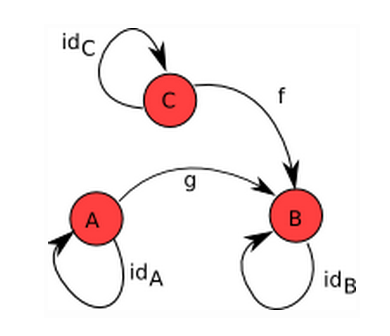
\includegraphics[scale=0.7]{functor.png}\\
\end{center}

In addition, there are three laws that categories must obey: associativity under morphism composition, closure of the category under composition, and the existence of an identity morphism for every object which is an identity under composition with any other morphism. (For details, see the Wikibooks page).\\

One of the most natural categories we can imagine is the category whose objects are sets and whose morphisms are simply all functions between sets. For Haskell, the category we are interested in is Hask, whose objects are all Haskell types and whose morphisms are Haskell functions. Thus a Haskell morphism is an ordinary function $f :: A -> B$. From this definition we can easily check that the three category laws are satisfied (the second through Haskell's (.) function composition and the third through Haskell's id function).\\

We can now define functors, which take categories to categories. In particular, a functor must act on both a category's objects and its morphisms; a functor must take any object in its domain to an object in its codomain, and it must take any morphism in its domain to a morphism in its codomain. In addition, $F$ must take an identity function of an object to the identity function of its image object, and $F(f \circ g)$ must equal $F(f) \circ F(g)$ for any morphisms $f, g$ in the domain.\\

Despite the relatively lengthy introduction so far, we will see that these properties are critical to understanding functors in Haskell, since they are defined in close alignment with this functor definition. In particular, in Haskell a functor is a map from the category Hask to one of its subcategories. Recalling that Hask is the category containing all Haskell types and functions between those types, we can now define a functor as a map between Hask and a subset of its types (and the functions between those types). For example, the list functor is a map from Hask to Lst, the subcategory containing just list types, as well as the associated functions which act on list types. \\

Perhaps a more interesting Haskell functor is the Maybe functor. How is this a functor? From our definitions, we know that to be a functor, it need only do two things: first, take the objects of the Hask category – that is, types – to other types, and second, to take functions between types to other functions between types. Looking at the code for the Maybe functor below,
\begin{verbatim}
class Functor (f :: * -> *) where
  fmap :: (a -> b) -> f a -> f b

instance Functor Maybe where
  fmap f (Just x) = Just (f x)
  fmap _ Nothing  = Nothing

\end{verbatim}

We see that the functor satisfies those two conditions. It takes any type T to a Maybe T, and fmap takes any function $A \rightarrow B$ and to a function $MaybeA \rightarrow Maybe B$. We can also check that the two additional axioms for functors are satisfied. Thus Maybe, as improbable as it may seem, is a functor.\\

Thus, in contrast to SML functors, which map structures to structures$^{5}$, Haskell functors map types to types (that preserves their corresponding functions), providing us with a notion of which types can be mapped over. In particular, a Haskell functor such as Maybe tells us that for any function between objects that we might have, we are provided a route to a corresponding function over the Maybe's of those objects.\\

\subsection*{Discussion}
In replicating the SML interpreter in Haskell we defined datatypes, and quickly realized that in defining Haskell datatypes we needed to also declare from which typeclasses our datatypes derived. For each datatype, therefore, we had to make a conscious decision about whether it belonged to the typeclass of things that could be compared for equality (Eq), whether it belonged to the typeclass of things that can be converted to character strings for I/O (Show), and so on. We found that the requirement of making these deliberate decisions to be illuminating, since in SML we generally did not have to think about these properties for datatypes except when creating modules.\\

In SML, we built a signature and a structure which define and implement a datatype called MyArray, which predictably implements an array-like data structure using SML lists. We then defined a signature for a linkedList type and built a functor which took the MyArray structure as a parameter and used the MyArray functions to construct the linkedList functions. One thing which after some time became very clear to us was the strength of the abstraction provided by the signature interface; while it was very tempting to access the list implementation of MyArray in order to create the list implementation of linkedList, it was impossible to do so, since the signature abstraction guaranteed us the behavior of the MyArray datatype without allowing us access to the implementation. Since the construction of the linkedList functions therefore required us to use the MyArray functions (implemented as lists), we ended up creating inefficient code whose writing process was nevertheless highly instructive.

\section{Conclusion}
Through our exploration of Haskell, we realized that while Haskell shares many commonalities with SML, the two programming languages are distinct in several ways, as outlined in our case study. Some of the strengths of Haskell are its purity and lazy evaluation. By separating the pure versus impure components of a program, code in Haskell becomes more compositional. In addition, Haskell's lazy evaluation means that expressions are evaluated once, at most, lending itself nicely to using infinite data structures. Haskell is also useful for concurrent programming due to its reliance on monads. \\
Through this project, we walked away not only with a better understanding of Haskell as a programming language, but with a greater understanding of the functional programming paradigm. 


% needed in second column of first page if using \IEEEpubid
%\IEEEpubidadjcol

% An example of a floating figure using the graphicx package.
% Note that \label must occur AFTER (or within) \caption.
% For figures, \caption should occur after the \includegraphics.
% Note that IEEEtran v1.7 and later has special internal code that
% is designed to preserve the operation of \label within \caption
% even when the captionsoff option is in effect. However, because
% of issues like this, it may be the safest practice to put all your
% \label just after \caption rather than within \caption{}.
%
% Reminder: the "draftcls" or "draftclsnofoot", not "draft", class
% option should be used if it is desired that the figures are to be
% displayed while in draft mode.
%
%\begin{figure}[!t]
%\centering
%\includegraphics[width=2.5in]{myfigure}
% where an .eps filename suffix will be assumed under latex, 
% and a .pdf suffix will be assumed for pdflatex; or what has been declared
% via \DeclareGraphicsExtensions.
%\caption{Simulation Results}
%\label{fig_sim}
%\end{figure}

% Note that IEEE typically puts floats only at the top, even when this
% results in a large percentage of a column being occupied by floats.


% An example of a double column floating figure using two subfigures.
% (The subfig.sty package must be loaded for this to work.)
% The subfigure \label commands are set within each subfloat command, the
% \label for the overall figure must come after \caption.
% \hfil must be used as a separator to get equal spacing.
% The subfigure.sty package works much the same way, except \subfigure is
% used instead of \subfloat.
%
%\begin{figure*}[!t]
%\centerline{\subfloat[Case I]\includegraphics[width=2.5in]{subfigcase1}%
%\label{fig_first_case}}
%\hfil
%\subfloat[Case II]{\includegraphics[width=2.5in]{subfigcase2}%
%\label{fig_second_case}}}
%\caption{Simulation results}
%\label{fig_sim}
%\end{figure*}
%
% Note that often IEEE papers with subfigures do not employ subfigure
% captions (using the optional argument to \subfloat), but instead will
% reference/describe all of them (a), (b), etc., within the main caption.


% An example of a floating table. Note that, for IEEE style tables, the 
% \caption command should come BEFORE the table. Table text will default to
% \footnotesize as IEEE normally uses this smaller font for tables.
% The \label must come after \caption as always.
%
%\begin{table}[!t]
%% increase table row spacing, adjust to taste
%\renewcommand{\arraystretch}{1.3}
% if using array.sty, it might be a good idea to tweak the value of
% \extrarowheight as needed to properly center the text within the cells
%\caption{An Example of a Table}
%\label{table_example}
%\centering
%% Some packages, such as MDW tools, offer better commands for making tables
%% than the plain LaTeX2e tabular which is used here.
%\begin{tabular}{|c||c|}
%\hline
%One & Two\\
%\hline
%Three & Four\\
%\hline
%\end{tabular}
%\end{table}


% Note that IEEE does not put floats in the very first column - or typically
% anywhere on the first page for that matter. Also, in-text middle ("here")
% positioning is not used. Most IEEE journals use top floats exclusively.
% Note that, LaTeX2e, unlike IEEE journals, places footnotes above bottom
% floats. This can be corrected via the \fnbelowfloat command of the
% stfloats package.







% if have a single appendix:
%\appendix[Proof of the Zonklar Equations]
% or
%\appendix  % for no appendix heading
% do not use \section anymore after \appendix, only \section*
% is possibly needed

% use appendices with more than one appendix
% then use \section to start each appendix
% you must declare a \section before using any
% \subsection or using \label (\appendices by itself
% starts a section numbered zero.)
%


% use section* for acknowledgement
\section*{Acknowledgment}


The authors would like to thank Ben Wood for his  help and insight throughout the development and implementation of this project. 


\section*{References}
\raggedright
$^{[1]}$Learn You a Haskell, the Monad Type Class, http://learnyouahaskell.com/a-fistful-of-monads\\
$^{[2]}$Learn You a Haskell, do notation, http://learnyouahaskell.com/a-fistful-of-monads\\
$^{[3]}$Example code gratefully borrowed from http://www.cs.cornell.edu/courses/cs312/2006fa/recitations/rec08.html\\
$^{[4]}$This detour borrows very heavily from the Wikibooks page “Haskell/Category Theory” at: http://en.wikibooks.org/wiki/Haskell/Category\_theory.\\
$^{[5]}$An interesting discussion on SML functors can be found at http://cs.stackexchange.com/questions/9769/what-is-the-relation-between-functors-in-sml-and-category-theory; essentially, it treats SML structures as algebras and considers whether these functors are functors in the category theoretic sense. Obviously there is a map between objects (structure to structure), but is there a map between morphisms? One response suggests not, as long as the structures contain higher-order operations, which category theory does not deal with.\\

\section*{Resources}

http://en.wikibooks.org/wiki/Haskell/Laziness\\
https://wiki.haskell.org/Functional\_programming\#Purity\_and\_effects\\
https://wiki.haskell.org/wikiupload/0/0a/TMR-Issue10.pdf

% Can use something like this to put references on a page
% by themselves when using endfloat and the captionsoff option.
\ifCLASSOPTIONcaptionsoff
  \newpage
\fi



% trigger a \newpage just before the given reference
% number - used to balance the columns on the last page
% adjust value as needed - may need to be readjusted if
% the document is modified later
%\IEEEtriggeratref{8}
% The "triggered" command can be changed if desired:
%\IEEEtriggercmd{\enlargethispage{-5in}}

% references section

% can use a bibliography generated by BibTeX as a .bbl file
% BibTeX documentation can be easily obtained at:
% http://www.ctan.org/tex-archive/biblio/bibtex/contrib/doc/
% The IEEEtran BibTeX style support page is at:
% http://www.michaelshell.org/tex/ieeetran/bibtex/
%\bibliographystyle{IEEEtran}
% argument is your BibTeX string definitions and bibliography database(s)
%\bibliography{IEEEabrv,../bib/paper}
%
% <OR> manually copy in the resultant .bbl file
% set second argument of \begin to the number of references
% (used to reserve space for the reference number labels box)


% biography section
% 
% If you have an EPS/PDF photo (graphicx package needed) extra braces are
% needed around the contents of the optional argument to biography to prevent
% the LaTeX parser from getting confused when it sees the complicated
% \includegraphics command within an optional argument. (You could create
% your own custom macro containing the \includegraphics command to make things
% simpler here.)
%\begin{biography}[{\includegraphics[width=1in,height=1.25in,clip,keepaspectratio]{mshell}}]{Michael Shell}
% or if you just want to reserve a space for a photo:



% You can push biographies down or up by placing
% a \vfill before or after them. The appropriate
% use of \vfill depends on what kind of text is
% on the last page and whether or not the columns
% are being equalized.

%\vfill

% Can be used to pull up biographies so that the bottom of the last one
% is flush with the other column.
%\enlargethispage{-5in}



% that's all folks
\end{document}


